\documentclass[xcolor=dvipsnames]{beamer}

\usepackage{setspace}
\usepackage{beamerthemesplit}
\usepackage{graphicx}
\usepackage{epstopdf}
\usepackage[english]{babel}
\usepackage[latin1]{inputenc}
\usepackage{times}
\usepackage[T1]{fontenc}
\usepackage{color}
\usepackage{colortbl}
\usepackage[noend]{algorithm,algpseudocode}
\usepackage{multimedia,xmpmulti}
\usepackage{multirow,multicol}
\usepackage[absolute,overlay]{textpos}
\usepackage{multimedia,xmpmulti}
\usepackage{tabularx,multicol}
\usepackage{url}
\usepackage{ulem}

%% ------------------------------------------------------------
%% PACKAGES
%% ------------------------------------------------------------

%% For \circledast
\usepackage{amssymb,amsfonts,amsmath}

%% For \mathscr
\usepackage[mathscr]{eucal}

%% For \llbracket and \rrbracket, \varoast, \varoslash
\usepackage{stmaryrd}

%% For \boldsymbol
\usepackage{amsbsy}

%% For \bm (bold math)
\usepackage{bm}

%% For \set, \Set
\usepackage{braket}

%% ------------------------------------------------------------
%% MACROS
%% ------------------------------------------------------------


%% --- Extras ---
% Transpose
\newcommand{\Tra}{{\sf T}} 
\newcommand{\parens}[1]{(#1)}
\newcommand{\Parens}[1]{\left(#1\right)}
\newcommand{\dsquare}[1]{\llbracket #1 \rrbracket}
\newcommand{\Dsquare}[1]{\left\llbracket #1 \right\rrbracket}
\newcommand{\curly}[1]{\{ #1 \}}
\newcommand{\Curly}[1]{\left\{ #1 \right\}}
\newcommand{\Real}{\mathbb{R}}
\newcommand{\qtext}[1]{\quad\text{#1}\quad}

%% --- Vectors ---
% vector
\newcommand{\V}[2][]{{\bm{#1\mathbf{\MakeLowercase{#2}}}}} 
% element of vector
\newcommand{\VE}[3][]{#1{\MakeLowercase{#2}}_{#3}} 
% vector in series
\newcommand{\Vn}[3][]{{\bm{#1\mathbf{\MakeLowercase{#2}}}}^{(#3)}} 
% transposed vector in series
\newcommand{\VnTra}[3][]{{\bm{#1\mathbf{\MakeLowercase{#2}}}}^{(#3)\Tra}} 
% element of vector in series
\newcommand{\VnE}[4][]{#1{\MakeLowercase{#2}}^{(#3)}_{#4}} 

%% --- Matrices ---
% matrix
\newcommand{\M}[2][]{{\bm{#1\mathbf{\MakeUppercase{#2}}}}} 
% matrix in series
\newcommand{\Mn}[3][]{{\bm{#1\mathbf{\MakeUppercase{#2}}}}^{(#3)}} 
% transposed matrix in series 
\newcommand{\MnTra}[4][]{{\bm{#1\mathbf{\MakeUppercase{#2}}}}^{(#3)\Tra}} 
% matrix column
\newcommand{\MC}[3][]{\V[#1]{#2}_{#3}} 
% column of matrix in series
\newcommand{\MnC}[4][]{\Vn[#1]{#2}{#3}_{#4}} 
% transposed column of matrix in series
\newcommand{\MnCTra}[4][]{\VnTra[#1]{#2}{#3}_{#4}} 
% matrix element
\newcommand{\ME}[3][]{#1{\MakeLowercase{#2}}_{#3}} 
% element of matrix in series
\newcommand{\MnE}[4][]{#1{\MakeLowercase{#2}}^{(#3)}_{#4}} 

%% --- Tensors ---
% tensor
\newcommand{\T}[2][]{\boldsymbol{#1\mathscr{\MakeUppercase{#2}}}} 
% tensor slide
\newcommand{\TS}[3][]{\M[#1]{#2}_{#3}}
% tensor element
\newcommand{\TE}[3][]{#1{\MakeLowercase{#2}}_{#3}}
% matriczied tensor
\newcommand{\Mz}[3][]{\M[#1]{#2}_{(#3)}}

%% --- Operators ---
% outer product
\newcommand{\Oprod}{\circ} 
% Kronecker product
\newcommand{\Kron}{\otimes} 
% Khatri-Rao product
\newcommand{\Khat}{\odot} 
% Hadamard (elementwise multiply)
\newcommand{\Hada}{\ast} 
\newcommand{\BigHada}{\mathop{\mbox{\fontsize{18}{19}\selectfont $\circledast$}}} 
% Elementwise divide
\newcommand{\Divi}{\varoslash}




%% Tikz - For making pretty pictures
\usepackage{tikz}
\usetikzlibrary{3d}
\usetikzlibrary{patterns}
\usetikzlibrary{calc}
\usetikzlibrary{arrows}

\usepackage{pgfplots}
\usepackage{pgfplotstable}
\usepackage{etoolbox}
%\pgfplotsset{compat=1.12}
\usetikzlibrary{decorations.pathreplacing}
\makeatletter
\newcommand{\gettikzxy}[3]{%
  \tikz@scan@one@point\pgfutil@firstofone#1\relax
  \edef#2{\the\pgf@x}%
  \edef#3{\the\pgf@y}%
}
\makeatother
\newcommand{\datafile}{}

\algrenewcommand{\algorithmiccomment}[1]{\textit{$\%$ #1}}
\newcommand{\lt}{\left}
\newcommand{\rt}{\right}
\newcommand{\ra}{\rightarrow}
\newcommand{\dis}{\displaystyle}
\newcommand{\bc}[3]{\left\langle#1, #2, #3\right\rangle}
\DeclareMathOperator*{\argmin}{arg\,min}
\newcommand{\ignore}[1]{}
\newtheorem{thm}{Theorem}
\newtheorem{lem}[thm]{Lemma}
\definecolor{bgblue}{rgb}{0.8,0.85,1}
\definecolor{bggreen}{rgb}{0.8,1,0.8}
\definecolor{bgred}{rgb}{1,0.85,0.8}
\definecolor{Blue}{rgb}{.08,0,.7}
\setbeamercolor{greentextbox}{fg=black,bg=bggreen}

\definecolor{wfugold}{rgb}{0.6196078,0.494117647,0.21960784}
\newcommand{\red}[1]{\textcolor{red}{#1}}
\newcommand{\blue}[1]{\textcolor{blue}{#1}}
\newcommand{\multiplycolor}{red}
\newcommand{\zero}{}
\newcommand{\cred}[1]{\textcolor{red}{#1}}
\newcommand{\cblue}[1]{\textcolor{blue}{#1}}
\newcommand{\cgold}[1]{\textcolor{wfugold}{#1}}

\newcommand{\UVW}{\llbracket \M U, \M V, \M W \rrbracket}
\newcommand{\plusequals}{\mathrel{+}=}
\algdef{SE}[FORDOTS]{ForDots}{EndForDots}{$\ddots$}{}


\graphicspath{{fig/}}

\mode<presentation>

\usetheme{Warsaw}
\usecolortheme[named=wfugold]{structure}
%Madrid
%\usecolortheme{dolphin}
%\useinnertheme{rounded}
%\usefonttheme{serif}
\setbeamertemplate{navigation symbols}{} % gets rid of navigation bars
\setbeamertemplate{footline}
{
  \hbox{
  \begin{beamercolorbox}[wd=.33\paperwidth,ht=2.25ex,dp=1ex,left]{author in head/foot}%
    \usebeamerfont{author in head/foot}
    Ballard
  \end{beamercolorbox}%
  \begin{beamercolorbox}[wd=.34\paperwidth,ht=2.25ex,dp=1ex,center]{title in head/foot}%
    \usebeamerfont{title in head/foot}
    
  \end{beamercolorbox}%
  \begin{beamercolorbox}[wd=.33\paperwidth,ht=2.25ex,dp=1ex,right]{date in head/foot}%
    \usebeamerfont{date in head/foot}
    \insertframenumber{} \hspace*{2ex} 
  \end{beamercolorbox}}%
}


\begin{document}

\title{Communication-Optimal Algorithms for \\ CP Decompositions of Dense Tensors}
\author[Ballard]{\textbf{Grey Ballard}, Koby Hayashi, Ramakrishnan Kannan, Nicholas Knight, Kathryn Rouse}
\institute{
\includegraphics[scale=.15]{wfulogo}}
\date{May 8, 2018}
\titlegraphic{SIAM Conference on Applied Linear Algebra \\ \small MS04: Constrained Low-Rank Matrix
and Tensor Approximations}
\begin{frame}[label=title,plain]
\maketitle
\end{frame}
\addtocounter{framenumber}{-1}

\begin{frame}[label=summary]
\frametitle{Summary}

\begin{itemize}
	\item We establish communication lower bounds for matricized-tensor times Khatri-Rao product (MTTKRP)
	\begin{itemize}
		\item key kernel for computing CP decomposition
	\end{itemize}
	\vfill
	\item We present optimal parallel dense MTTKRP algorithm
	\begin{itemize}
		\item attains the lower bound to within constant factors
	\end{itemize}
	\vfill
	\item We implement and benchmark optimal CP-ALS algorithm
	\begin{itemize}
		\item remains computation bound and scales well
		\item dimension tree optimization avoids redundant computation
	\end{itemize}
\end{itemize}

\end{frame}



\begin{frame}
\frametitle{CP Decomposition: sum of outer products}

Matrix: \quad $\displaystyle \M{M} \approx \sum_{r=1}^R \MC{U}{r} (\sigma_r \MC{V}{r}^T)$
\begin{center}
\scalebox{.14}{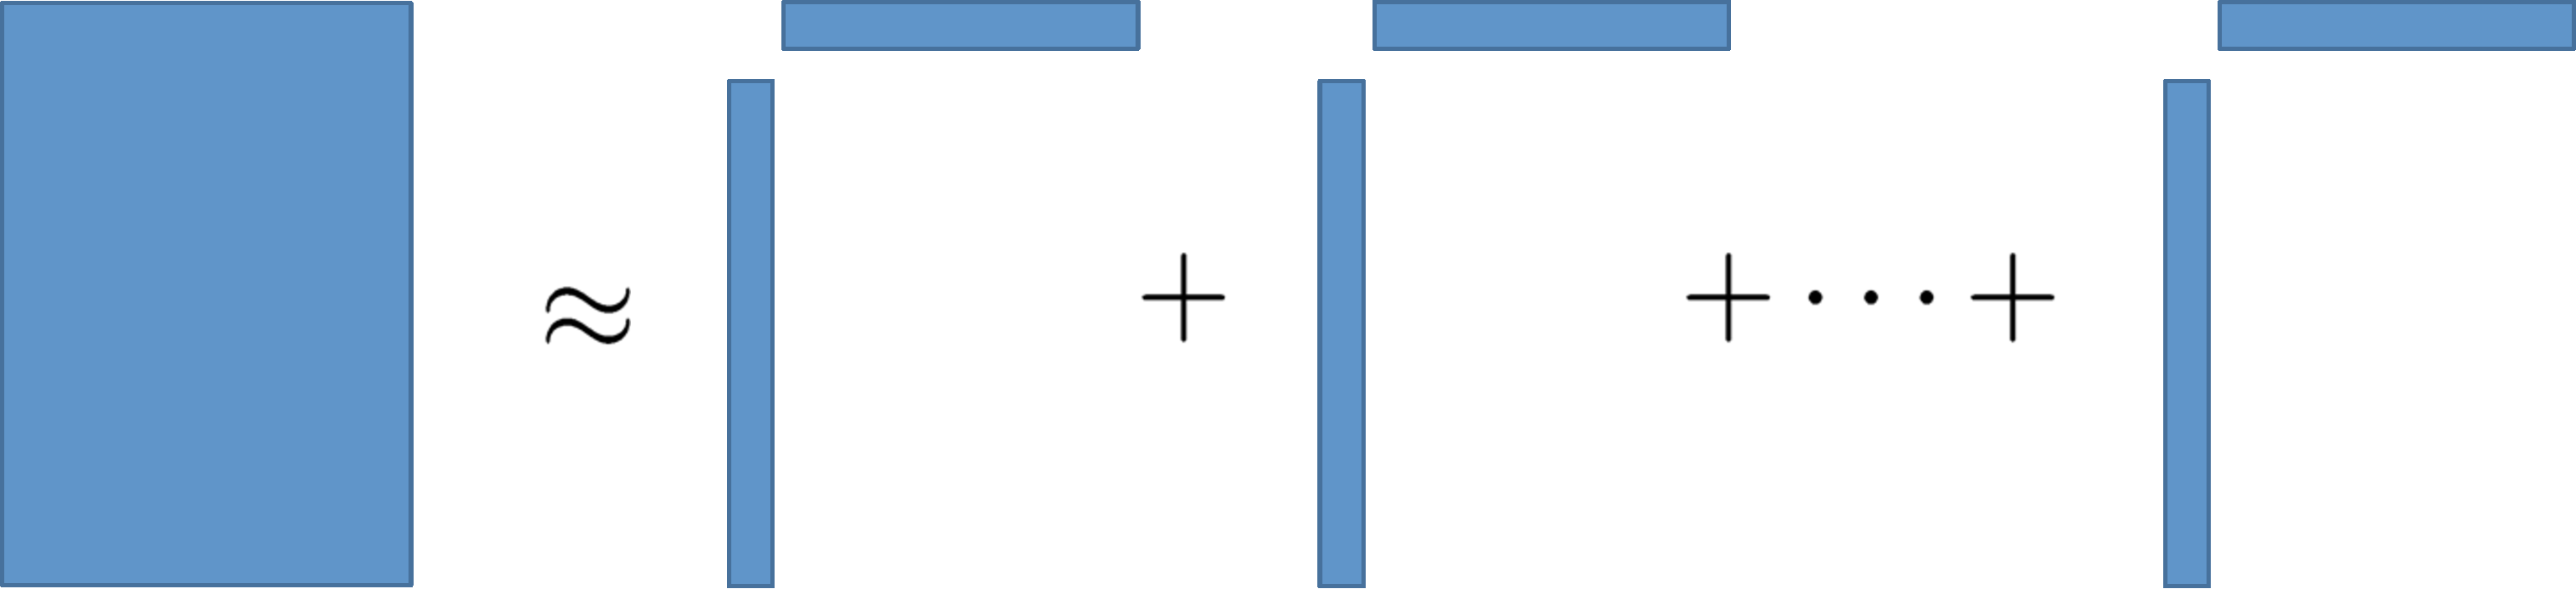
\includegraphics{matrix-LR-SOP}}
\end{center}
\vfill
Tensor: \quad $\displaystyle \T{X}\approx \sum_{r=1}^R \MC{U}{r}\circ\MC{V}{r}\circ\MC{W}{r}$
\begin{center}
\scalebox{.27}{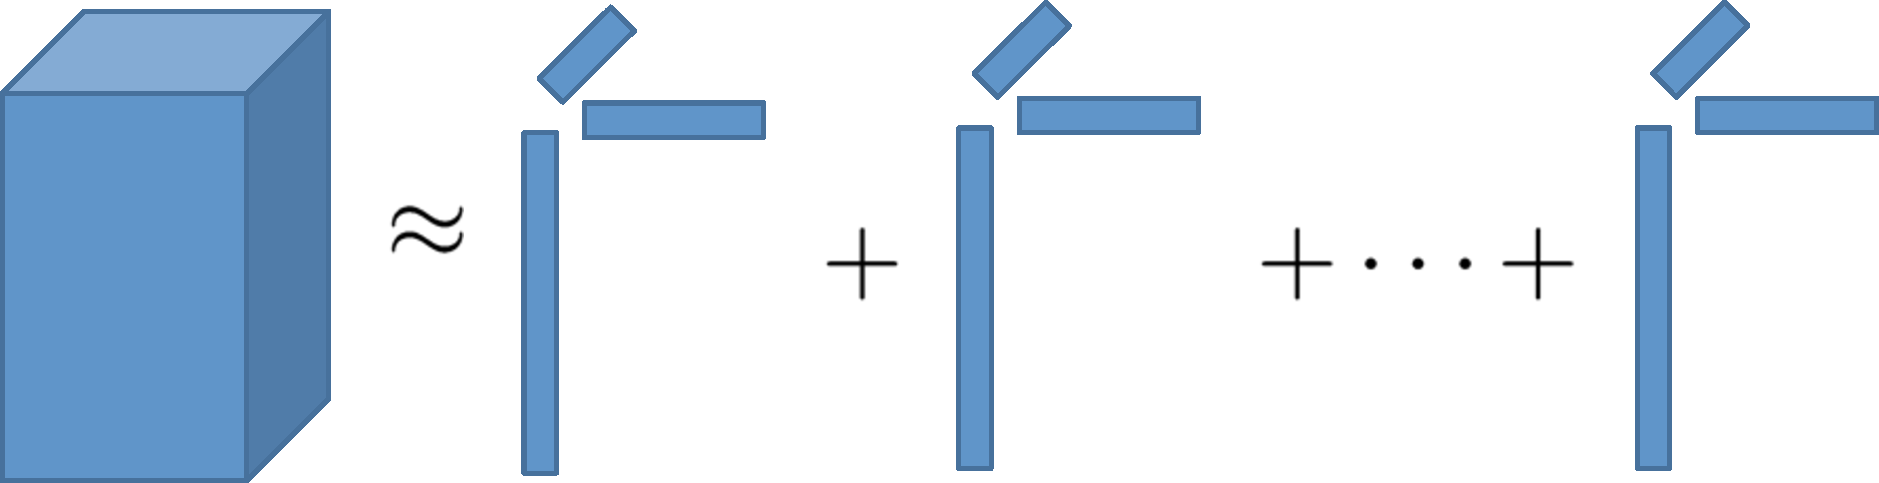
\includegraphics{tensor-LR-SOP}}
\end{center}
\vfill
\begin{center}
This is known as the CANDECOMP or PARAFAC or \\ canonical polyadic or \textcolor{wfugold}{CP decomposition}
\end{center}

\end{frame}

\begin{frame}
\frametitle{CP Optimization Problem}

\begin{center}
\scalebox{.15}{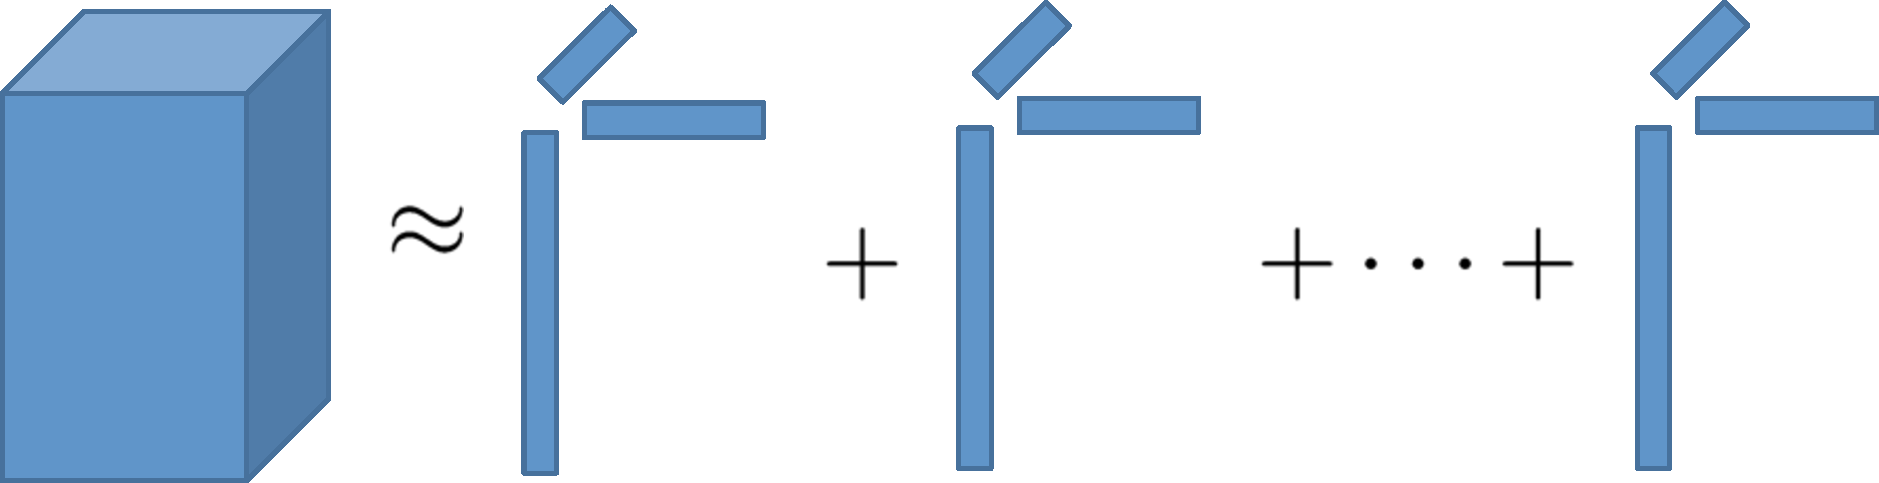
\includegraphics{tensor-LR-SOP}}
\end{center}
\vfill
\begin{flushleft} 
For fixed rank $R$, we want to solve
\end{flushleft}
%\vspace{-1.5cm}
$$\min_{\M{U},\M{V},\M{W}} \left\|\T{X}-\sum_{r=1}^R \MC{U}{r}\circ\MC{V}{r}\circ\MC{W}{r}\right\| $$
\vfill
\begin{flushright}
which is a nonlinear, nonconvex optimization problem
\end{flushright}
\vfill
{\small 
\begin{itemize}
	\item in the matrix case, the SVD gives us the optimal solution
	\item in the tensor case, need iterative optimization scheme
\end{itemize}
}

\end{frame}

\begin{frame}
\frametitle{Alternating Least Squares (ALS)}

Fixing all but one factor matrix, we have a linear LS problem:
$$\min_{\M{V}} \left\|\T{X}-\sum_{r=1}^R \MC[\hat]{U}{r}\circ\MC{V}{r}\circ\MC[\hat]{W}{r}\right\| $$
or equivalently
$$\min_{\M{V}} \left\|\Mz{X}{2}-\M{V}(\M[\hat]{W} \Khat \M[\hat]{U})^\Tra\right\|_F $$

\begin{center}

\vfill

$\Khat$ is the \emph{Khatri-Rao} product, a column-wise Kronecker product or row-wise Hadamard (element-wise) product

\vfill

ALS works by alternating over factor matrices, updating one at a time by solving the corresponding linear LS problem

\end{center}

\end{frame}

\begin{frame}
\frametitle{CP-ALS}

\textbf{Repeat}
\begin{enumerate}
	\item Solve $\M{U}(\M{V}^\Tra\M{V} \Hada \M{W}^\Tra\M{W}) = \textcolor{wfugold}{\Mz{X}{1}(\M{W} \Khat \M{V})}$ for $\M{U}$ 
	%\item Normalize columns of $\M{U}$
	\item Solve $\M{V}(\M{U}^\Tra\M{U} \Hada \M{W}^\Tra\M{W}) = \textcolor{wfugold}{\Mz{X}{2}(\M{W} \Khat \M{U})}$ for $\M{V}$ 
	%\item Normalize columns of $\M{V}$
	\item Solve $\M{W}(\M{U}^\Tra\M{U} \Hada \M{V}^\Tra\M{V}) = \textcolor{wfugold}{\Mz{X}{3}(\M{V} \Khat \M{U})}$ for $\M{W}$ 
	%\item Normalize columns of $\M{W}$ and store norms in $\V{\lambda}$
\end{enumerate}

\vfill

\begin{center}
{\small
Linear least squares problems solved via normal equations \\ using identity $(\M{A}\Khat\M{B})^\Tra(\M{A}\Khat\M{B}) = \M{A}^\Tra\M{A} \Hada \M{B}^\Tra\M{B}$, \\ where $\Hada$ is Hadamard product
\vfill
All optimization schemes that compute the gradient \\ must also compute \textcolor{wfugold}{MTTKRP} in all modes: e.g.,
$$\frac{\partial f}{\partial \M{V}} = \M{V}(\M{U}^\Tra\M{U} \Hada \M{W}^\Tra\M{W}) - \textcolor{wfugold}{\Mz{X}{2}(\M{W} \Khat \M{U})}$$
}
\end{center}

\end{frame}

\begin{frame}
\frametitle{MTTKRP bottleneck}

\begin{itemize}
	\item How do we compute MTTKRP efficiently?
	\vfill
	\item How do we parallelize MTTKRP efficiently?
	\begin{itemize}
		\item how do we load balance computation?
		\item how do we minimize communication?
	\end{itemize}
\end{itemize}

\end{frame}

\begin{frame}
\frametitle{MTTKRP via Matrix Multiplication}

$$\text{MTTKRP:  } \quad \textcolor{wfugold}{\M{M} = \Mz{X}{2}(\M{W} \Khat \M{U})}$$

\vfill

Standard approach to MTTKRP for dense tensors
\begin{enumerate}
	\item ``form'' matricized tensor (a matrix)
	\item compute Khatri-Rao product (a matrix)
	\item call matrix-matrix multiplication subroutine
\end{enumerate}

\vfill

\begin{center}
Can we communicate less by exploiting tensor structure? \\ (avoiding forming explicit Khatri-Rao product)
\end{center}

\end{frame}

\begin{frame}
\frametitle{MTTKRP for \only<1>{3}\only<2>{$N$}-way Tensors}

\textbf{Matrix equation}:  
\only<1>{$$\M{M} = \Mz{X}{2}(\M{W} \Khat \M{U})$$}
\only<2>{$$\Mn{M}{n} = \Mz{X}{n}(\Mn{U}{N} \Khat \cdots \Khat \Mn{U}{n+1} \Khat \Mn{U}{n-1} \Khat \cdots \Khat \Mn{U}{1})$$}

\vfill

\textbf{Element equation}:  
\only<1>{$$\ME{M}{jr} = \sum_{i=1}^I \sum_{k=1}^K \TE{X}{ijk} \ME{U}{ir} \ME{W}{kr}$$}
\only<2>{$$\MnE{M}{n}{i_nr} = \sum \TE{X}{i_1\dots i_N} \prod_{m\neq n} \MnE{U}{m}{i_mr} $$}

\vfill

\textbf{Example pseudocode}:

\begin{center}
\begin{algorithmic}
\only<1>{
\For{$i=1$ to $I$}
	\For{$j=1$ to $J$}
		\For{$k=1$ to $K$}
			\For{$r=1$ to $R$}
				\State $\M M(j,r) \plusequals \T{X}(i,j,k) \cdot \M{U}(i,r) \cdot \M{W}(k,r)$
			\EndFor
		\EndFor
	\EndFor
\EndFor
}\only<2>{
\For{$i_1=1$ to $I_1$}
	\ForDots
		\For{$i_N=1$ to $I_N$}
			\For{$r=1$ to $R$}
				\State \footnotesize $\Mn{M}{n}(i_n,r) \plusequals \T{X}(i_1,\dots,i_N) \cdot \Mn{U}{1}(i_1,r)  \cdots  \Mn{U}{N}(i_N,r)$
			\EndFor
		\EndFor
	\EndForDots
\EndFor
}
\end{algorithmic}
\end{center}

\end{frame}

\begin{frame}
\frametitle{Communication Lower Bounds for MTTKRP}

MTTKRP is a set of nested loops that accesses arrays
\begin{itemize}
	\small
	\item Nick's PhD thesis was ``Communication-Optimal Loop Nests"
	\item References: thesis \cite{Knight15} and paper \cite{CDKSY13}
\end{itemize}

\vfill

From Nick's thesis...
\begin{itemize}
	\item tabulate how the arrays are accessed
	\item use H\"{o}lder-Brascamp-Lieb-type inequality in LB proof
	\item solve linear program to get tightest lower bound
\end{itemize}

\end{frame}

\begin{frame}
\frametitle{MTTKRP Lower Bound Proofs}

\begin{itemize}
	\item Lower bound argument follows \cite{CDKSY13} almost directly
	%\begin{itemize}
	%	\item solve linear program involving $\Delta$ for tightest bound
	%\end{itemize}
	\vfill
	\pause
	\item Gotcha: the number of nested loops is not constant
	\begin{itemize}
		%\item LB becomes too low by a factor of $O(N)$ (number of loops)
		\item Fixed using a technique similar to one used for tightening the constant in matrix multiplication lower bound \cite{SvdG17}
	\end{itemize}
	\vfill
	\pause
	\item Gotcha: memory-independent bounds most relevant
	\begin{itemize}
		\item inspiration from matrix multiplication \cite{BDHLS12-SS,DE+13}
	\end{itemize}
	\vfill
	\pause
	\item Key assumption: algorithm is not allowed to pre-compute and re-use temporary values 
	\begin{itemize}
		\item e.g., forming explicit Khatri-Rao product
		\item e.g., computing and re-using ``partial'' MTTKRP
	\end{itemize}
\end{itemize}

\end{frame}



\begin{frame}
\frametitle{Parallel Communication Lower Bound}

\begin{theorem}
Any parallel MTTKRP algorithm involving a tensor with $I_k=I^{1/N}$ for all $k$ and that evenly distributes one copy of the input and output performs at least
\begin{equation*}
\Omega\left( \left( \frac{NIR}{P} \right)^{\frac{N}{2N-1}} + NR\left(\frac{I}{P}\right)^{1/N} \right)
\end{equation*}
sends and receives.  (Either term can dominate.)
\end{theorem}

\vfill

\small
\begin{itemize}
	\footnotesize
	\item $N$ is the number of modes
	\item $I$ is the number of tensor entries
	\item $I_k$ is the dimension of the $k$th mode
	\item $R$ is the rank of the CP model
	\item $P$ is the number of processors
\end{itemize}

\end{frame}

\begin{frame}
\frametitle{Communication-Optimal Parallel Algorithm (3D)}

\begin{columns}

\begin{column}{.6\textwidth}

\newcommand{\procdim}{3}
\newcommand{\proc}{\draw[black,shift={(-.5,-.5)}] (0,0) grid (\procdim,\procdim);}
\newcommand{\highlight}{gray!75}
\newcommand{\commhighlight}{gray!25}

\begin{center}
\begin{tikzpicture}[x={(-0.5cm,-0.4cm)}, y={(1cm,0cm)}, z={(0cm,1cm)},every node/.append style={transform shape}]

% highlight all-gather/reduce-scatter patterns
% 1st slide is proc data (leave highlighting for all slides)
% 2nd slide is all-gather in 1st mode
\only<2>{
% front face
\begin{scope}[canvas is yz plane at x=.5]
	% highlight front face of proc comm
	\draw[fill=\commhighlight,shift={(-.5,-.5)}] (0,0) rectangle (3,1);
	% highlight block of 1st factor matrix
	\draw[fill=\commhighlight,shift={(-1,.5)},xscale=.5] (0,0) rectangle (-1,-1);
\end{scope}
% right face
\begin{scope}[canvas is zx plane at y=(\procdim-.5),rotate=-90]
	% highlight right face of proc comm
	\draw[fill=\commhighlight,shift={(-.5,-.5)}] (0,0) rectangle (3,1);
\end{scope}
% top face
\begin{scope}[canvas is yx plane at z=.5,yscale=-1,rotate=0]
	% highlight top face of proc comm
	\draw[fill=\commhighlight,shift={(-.5,-.5)}] (0,0) rectangle (3,3);
\end{scope}
}
% 3rd slide is all-gather in 3rd mode
\only<3>{
% front face
\begin{scope}[canvas is yz plane at x=.5]
	% highlight front face of proc comm
	\draw[fill=\commhighlight,shift={(-.5,.5)}] (0,0) rectangle (3,-3);
	% highlight block of 1st factor matrix now owned by processor
	\draw[fill=\highlight,shift={(-1,.5)},xscale=.5] (0,0) rectangle (-1,-1);
\end{scope}
% right face
\begin{scope}[canvas is zx plane at y=(\procdim-.5),rotate=-90]
	% highlight right face of proc comm
	\draw[fill=\commhighlight,shift={(-.5,.5)}] (0,0) rectangle (1,-3);
	% highlight block of 3rd factor matrix
	\draw[fill=\commhighlight,yscale=.5,shift={(-.5,-6)}] (0,0) rectangle (1,-1);
\end{scope}
% top face
\begin{scope}[canvas is yx plane at z=.5,yscale=-1,rotate=0]
	% highlight top face of proc comm
	\draw[fill=\commhighlight,shift={(-.5,-.5)}] (0,0) rectangle (3,1);
\end{scope}
}
% 4th and 5th slides are local computation
\only<4-5>{
% front face
\begin{scope}[canvas is yz plane at x=.5]
	% highlight block of 1st factor matrix now owned by processor
	\draw[fill=\highlight,shift={(-1,.5)},xscale=.5] (0,0) rectangle (-1,-1);
\end{scope}
% right face
\begin{scope}[canvas is zx plane at y=(\procdim-.5),rotate=-90]
	% highlight block of 3rd factor matrix now owned by processor
	\draw[fill=\highlight,yscale=.5,shift={(-.5,-6)}] (0,0) rectangle (1,-1);
\end{scope}
}
\only<5>{
% front face
\begin{scope}[canvas is yz plane at x=.5]
	% highlight block of 2nd factor matrix contribution computed by processor
	\draw[fill=\highlight,shift={(1.5,-3)},yscale=.5] (0,0) rectangle (1,-1);
\end{scope}
}
% 6th slide is reduce-scatter in 2nd mode
\only<6>{
% front face
\begin{scope}[canvas is yz plane at x=.5]
	% highlight front face of proc comm
	\draw[fill=\commhighlight,shift={(1.5,.5)}] (0,0) rectangle (1,-3);
	% highlight block of 2nd factor matrix involved in reduce scatter
	\draw[fill=\commhighlight,shift={(1.5,-3)},yscale=.5] (0,0) rectangle (1,-1);
	% highlight block of 2nd factor matrix of computed output
	\draw[fill=\highlight,shift={(1.5,-3)},yscale=.5] (0,0) rectangle (1/9,-1);
	% highlight block of 1st factor matrix now owned by processor
	\draw[fill=\highlight,shift={(-1,.5)},xscale=.5] (0,0) rectangle (-1,-1);
\end{scope}
% right face
\begin{scope}[canvas is zx plane at y=(\procdim-.5),rotate=-90]
	% highlight right face of proc comm
	\draw[fill=\commhighlight,shift={(-.5,.5)}] (0,0) rectangle (3,-3);
	% highlight block of 3rd factor matrix now owned by processor
	\draw[fill=\highlight,yscale=.5,shift={(-.5,-6)}] (0,0) rectangle (1,-1);
\end{scope}
% top face
\begin{scope}[canvas is yx plane at z=.5,yscale=-1,rotate=0]
	% highlight top face of proc comm
	\draw[fill=\commhighlight,shift={(1.5,-.5)}] (0,0) rectangle (1,3);
\end{scope}
}

% highlight one processor's data
% front face
\begin{scope}[canvas is yz plane at x=.5,shift={(1.5,-1.5)}]
	% highlight front face of tensor block
	\draw[fill=\highlight,shift={(0,1)}] (0,0) rectangle (1,1);
	% highlight block of 1st factor matrix
	\draw[fill=\highlight,shift={(-2.5,2-1/3)},xscale=.5] (0,0) rectangle (-1,-1/9);
	% highlight block of 2nd factor matrix
	\draw[shift={(0,-1.5)},yscale=.5] (0,0) rectangle (1/9,-1);
\end{scope}
% right face
\begin{scope}[canvas is zx plane at y=(\procdim-.5),rotate=-90,shift={(-.5,-3)}]
	% highlight front face of tensor block
	\draw[fill=\highlight,shift={(0,2.5)}] (0,0) rectangle (1,1);
	% highlight block of 3rd factor matrix
	\draw[fill=\highlight,yscale=.5] (0,0) rectangle (1/9,-1);
\end{scope}
% top face
\begin{scope}[canvas is yx plane at z=.5,yscale=-1,rotate=0]
	% highlight front face of tensor block
	\draw[fill=\highlight,shift={(1.5,-.5)}] (0,0) rectangle (1,1);
\end{scope}

% draw tensor
% front face
\begin{scope}[canvas is yz plane at x=.5,rotate=-90]
	\proc
\end{scope}
% top face
\begin{scope}[canvas is yx plane at z=.5,yscale=-1,rotate=0]
	\proc
\end{scope}
% right face
\begin{scope}[canvas is zx plane at y=(\procdim-.5),rotate=180]
	\proc
\end{scope}

% draw factor matrices
% front face
\begin{scope}[canvas is yz plane at x=.5,shift={(1.5,-.5)}]
	% draw 1st factor matrix
	\draw[shift={(-2.5,0)},xscale=.5] (0,-2) grid (-1,1);
	\node[draw=none] at (-3.5,-.5) {$\Mn{U}{1}$};
	% draw 2nd factor matrix
	\draw[shift={(0,-2.5)},yscale=.5] (-2,0) grid (1,-1);
	\node[draw=none] at (-.5,-3.5) {$\Mn{M}{2}$};
\end{scope}
% right face
\begin{scope}[canvas is zx plane at y=(\procdim-.5),rotate=-90,shift={(1.5,-.5)}]
	% draw 2nd factor matrix
	\draw[shift={(0,-2.5)},yscale=.5] (-2,0) grid (1,-1);
	\node[draw=none] at (-.5,-3.5) {$\Mn{U}{3}$};
\end{scope}


\end{tikzpicture}
\end{center}

\end{column}
\begin{column}{.45\textwidth}

\footnotesize
Each processor
\begin{enumerate}
	\item Starts with one subtensor and subset of rows of each input factor matrix
	\uncover<2->{\item All-Gathers all the rows needed from $\Mn{U}{1}$}
	\uncover<3->{\item All-Gathers all the rows needed from $\Mn{U}{3}$}
	\uncover<4->{\item Computes its contribution to rows of $\Mn{M}{2}$ (local MTTKRP)}
	\uncover<6->{\item Reduce-Scatters to compute and distribute $\Mn{M}{2}$ evenly}
\end{enumerate}

\end{column}

\end{columns}

\end{frame}

\begin{frame}
\frametitle{Theoretical Comparisons}

\begin{center}
%\renewcommand{\arraystretch}{2}
\begin{tabular}{|c|ccc|}
\hline
& \textbf{Lower Bound} & \textbf{New Algorithm} & \textbf{Standard (MM$^*$)}  \\
\hline
\textbf{Words} & \multirow{2}{*}{$\Omega\left( NR\left(\frac IP \right)^{1/N} \right)$} & \multirow{2}{*}{$O\left(NR\left(\frac IP \right)^{1/N} \right)$} & \multirow{2}{*}{$O\left( I^{1/N}R \right)$} \\
\small (``small'' $P$) & & & \\
\hline
\uncover<2>{\textbf{Words}} & \uncover<2>{\multirow{2}{*}{$\Omega\left(\left(\frac{NIR}{P}\right)^{\frac{N}{2N-1}} \right)$} & \multirow{2}{*}{$O\left( \left(\frac{NIR}{P}\right)^{\frac{N}{2N-1}}  \right)$} & \multirow{2}{*}{$O\left( \left(\frac{IR}{P}\right)^{2/3} \right)$}} \\
\uncover<2>{\small (``large'' $P$)} & & & \\
\hline
\end{tabular}
\end{center}

\begin{itemize}
	\small
	\item For relatively small $P$ (or small $R$) and even dimensions, parallel ``stationary'' algorithm attains lower bound
	\begin{itemize}
		\small
		\item same algorithm for sparse \cite{SK16} and dense 3D \cite{LK+17b} 
	\end{itemize}
	\pause
	\item For larger $P$ (or $R$), then we need more general algorithm to attain lower bound
	\begin{itemize}
	%	\item also parallelize over columns of output matrix
		\item involves communicating the tensor
	\end{itemize}
%	\item Simple version of this parallel algorithm in \cite{LK+17}
\end{itemize}

\vfill

\begin{center}
\small 
$^*$communication-optimal matrix multiplication from \cite{DE+13}
\end{center}

\end{frame}

\begin{frame}
\frametitle{Modeled Communication Costs}

\begin{center}
%!TEX root = ../talk.tex

\begin{tikzpicture}[scale=.8]
\renewcommand{\datafile}{data/modeled.dat}
\begin{axis}[
	title=Modeled Strong-Scaling Comparison,
	xlabel=Processors,
	ylabel=Words Communicated,
	width=\columnwidth,
	xmode=log,
	log basis x={2},
	xmin=1,xmax=2^31,
	xtick={1,32,1024,32768,1048576,33554432,1073741824},
	ymode=log,
	legend pos=south west
	]
	\addplot [black,thick,dashed,mark options={solid},mark=x] table [x={P}, y={MM}] {\datafile};
	\addlegendentry{Matrix Multiplication}
	\addplot [red,thick,dashed,mark options={solid},mark=asterisk] table [x={P}, y={Alg3}] {\datafile};
	\addlegendentry{Stationary Tensor}
	\addplot [blue,thick,dashed,mark options={solid},mark=o] table [x={P}, y={Alg4}] {\datafile};
	\addlegendentry{General Tensor}
\end{axis}
\end{tikzpicture}

\end{center}

\end{frame}

\begin{frame}
\frametitle{What about for a full CP-ALS iteration?}

A full iteration of CP-ALS includes computing all $N$ MTTKRPs

\vfill

\textbf{Lower Bound}\\
Lower bound for single MTTKRP applies to computing all $N$

\vfill

\textbf{Algorithm}\\
We can compute all $N$ with same communication as just 1
\begin{itemize}
	\small
	\item lots of data overlap across MTTKRPs
	\item more computation required, but not that much more
\end{itemize}

\end{frame}

\begin{frame}
\frametitle{Avoiding re-communication across MTTKRPs}

\begin{algorithmic}
\While{not converged}
	\For{$n=1$ to $N$}
		\State \Comment{Compute new factor matrix in $n$th mode}
		\State \textcolor{wfugold}{$\M{M} = \text{Local-MTTKRP}(\T{X}_{p_1\cdots p_N},\{\Mn{U}{i}_{p_i}\},n)$}
		\State \textcolor{wfugold}{$\Mn{M}{n}_{\V{p}} = \text{Reduce-Scatter}(\M{M},\textsc{Proc-Slice}(n,\VE{p}{n}))$} 
		\State \textcolor{gray}{$\Mn{S}{n} = \Mn{G}{1} \Hada \cdots \Hada \Mn{G}{n-1} \Hada \Mn{G}{n+1} \Hada \cdots \Hada \Mn{G}{N}$}
		\State \textcolor{gray}{$\Mn{U}{n}_{\V{p}} = \text{Local-Update}(\Mn{S}{n},\Mn{M}{n}_{\V{p}})$}
		\State \Comment{Organize data for later modes}
		\State \textcolor{gray}{$\M{H} = {\Mn{U}{n}_{\V{p}}}^\Tra\Mn{U}{n}_{\V{p}}$}
		\State \textcolor{gray}{$\Mn{G}{n} = \text{All-Reduce}(\M{H},\textsc{All-Procs})$}
		\State \textcolor{wfugold}{$\Mn{U}{n}_{p_n} = \text{All-Gather}(\Mn{U}{n}_{\V{p}},\textsc{Proc-Slice}(n,\VE{p}{n}))$}
	\EndFor 
\EndWhile
\end{algorithmic}

\vfill

\begin{center}
\footnotesize
Compute factor matrix, communicate it \textbf{once} for use in all other $N{-}1$ modes
\end{center}

\end{frame}

\begin{frame}
\frametitle{Avoiding recomputation across MTTKRPs}

\footnotesize
We re-use communication \emph{and} computation across MTTKRPs
\normalsize
$$\Mn{M}{1}=\underline{\Mz{X}{1}\left(\Mn{U}{3}\rt.}\Khat\lt.\Mn{U}{2}\rt) \hspace{.5cm} \text{  and  } \hspace{.5cm} \Mn{M}{2}=\underline{\Mz{X}{2}\lt(\Mn{U}{3}\rt.}\Khat\lt.\Mn{U}{1}\rt)$$

\vfill
\pause

\footnotesize
We organize intermediate values in ``dimension tree'' \cite{PTC13a,LCPSV17,KU18}
\normalsize

\only<2>{
\begin{center}
\begin{tikzpicture}

\node (123) at (4,2) {$\{1,2,3\}$};
\node (12) at (2,1) {$\{1,2\}$};
\node (3) at (6,1) {$\Mn{M}{3}$};
\node (1) at (1,0) {$\Mn{M}{1}$};
\node (2) at (3,0) {$\Mn{M}{2}$};

\scriptsize
\path[draw] (123) edge [left,align=right] node {PM} (12);
\path[draw] (123) edge [right,align=left] node {PM} (3);
\path[draw] (12) edge [left,align=right] node {mTTV} (1);
\path[draw] (12) edge [right,align=left] node {mTTV} (2);
\normalsize

\end{tikzpicture}
\end{center}
}\only<3>{
\begin{center}
\begin{tikzpicture}

\node (12345) at (4,2) {$\{1,2,3,4,5\}$};
\node (12) at (2,1) {$\{1,2\}$};
\node (345) at (6,1) {$\{3,4,5\}$};
\node (1) at (1,0) {$\Mn{M}{1}$};
\node (2) at (3,0) {$\Mn{M}{2}$};
\node (3) at (5,0) {$\Mn{M}{3}$};
\node (45) at (7,0) {$\{4,5\}$};
\node (4) at (6,-1) {$\Mn{M}{4}$};
\node (5) at (8,-1) {$\Mn{M}{5}$};

\scriptsize
\path[draw] (12345) edge [left,align=right] node {PM} (12);
\path[draw] (12345) edge [right,align=left] node {PM} (345);
\path[draw] (12) edge [left,align=right] node {mTTV} (1);
\path[draw] (12) edge [right,align=left] node {mTTV} (2);
\path[draw] (345) edge [left,align=right] node {mTTV} (3);
\path[draw] (345) edge [right,align=left] node {mTTV} (45);
\path[draw] (45) edge [left,align=right] node {mTTV} (4);
\path[draw] (45) edge [right,align=left] node {mTTV} (5);
\normalsize

\end{tikzpicture}
\end{center}
}

\only<2-3>{
\begin{textblock}{15}(2.5,14.5)
\footnotesize
PM = Partial MTTKRP \hspace{1cm} mTTV = multi-Tensor-Times-Vector
\end{textblock}
}

\end{frame}

\begin{frame}
\frametitle{Implementation}

\begin{itemize}
	\item Uses CP-ALS for non-negative CP problems
	\begin{itemize}
		\item minimize least squares loss function
		\item use block principal pivoting \cite{KP11} to solve subproblems
	\end{itemize}
	\vfill
	\item Avoids redundant communication across MTTKRPs
	\vfill
	\item Avoids redundant computation across MTTKRPs \\ using dimension trees 
\end{itemize}

\end{frame}

% input file with plotting macros
% !TEX root = experiments.tex

% macros for plotting
\newcommand{\datafile}{}
\newcommand{\alg}{}
\newcommand{\numiterations}{30}
\newcommand{\minvalue}{1}

% toggles whether or not to plot naive results (if not, the rows of the data file also need to be commented out)
\newif\ifnaive
% toggles ksweep vs scaling plot
\newif\ifksweep
% toggles legend
\newif\iflegend
% toggles y axis label
\newif\ifylabel
% toggles wider plot area
\newif\ifwider
% toggles including liavas results
\newif\ifliavas


\newcommand{\setcolors}{
\pgfplotsset{cycle list={
	red, fill=red \\ 
	blue, fill=blue \\ 
	green, fill=green \\ 
	red, pattern=crosshatch, pattern color=red \\
	green, pattern=crosshatch, pattern color=green \\
	blue, pattern=crosshatch, pattern color=blue \\
}};
}

% set options for grouped bar plot
\newcommand{\breakdownplotoptions}{
	ybar stacked,
	reverse legend,
	bar width=8pt,
	width=9cm, height=3.85cm,
	ylabel={Time (s)}, 
	y label style={yshift=-.5cm},
	ymin=0,
	symbolic x coords={D1,N1,D16,N16,D81,N81,D256,N256},
	xtick=data,
	legend style={at={(0.5,1.3)},anchor=north},
	legend columns=-1,
	reverse legend
}

% stacked bar plot command
\newcommand{\breakdownplot}{
\begin{axis}[\breakdownplotoptions]
	\setcolors
	\addplot table[x=alg-p, y expr=(\thisrow{mttkrp}/(\minvalue*\numiterations))] {\datafile};
	\addplot table[x=alg-p, y expr=(\thisrow{krp}/(\minvalue*\numiterations))] {\datafile};
	\addplot table[x=alg-p, y expr=((\thisrow{allgather}+\thisrow{reducescatter})/(\minvalue*\numiterations))] {\datafile};
	\addplot table[x=alg-p, y expr=((\thisrow{nnls}+\thisrow{gram}+\thisrow{allreduce})/(\minvalue*\numiterations))] {\datafile};
	\addplot table[x=alg-p, y expr=((\thisrow{err_compute}+\thisrow{err_communication})/(\minvalue*\numiterations))] {\datafile};
	\legend{MTTKRP,KRP,Factor Comm,NLS,Error};
\end{axis}
}

% labels for bar groups (manually positioned)
\newcommand{\labels}{
%\node [align=center,text width=3cm] at (1.25cm, -.95cm)   {\ifksweep 10 \else 16 \fi};
%\node [align=center,text width=3cm] at (3cm, -0.95cm)   {\ifksweep 20 \else 96 \fi};
%\node [align=center,text width=3cm] at (4.6cm, -0.95cm)   {\ifksweep 30 \else 384 \fi};
%\node [align=center,text width=3cm] at (6.3cm, -0.95cm) {\ifksweep 40 \else 864 \fi};
%\node [align=center,text width=3cm] at (8.15cm, -0.95cm) {\ifksweep 50 \else 1536 \fi};
\node [align=center,text width=3cm] at (1cm, -1.15cm)   {\ifksweep 10 \else 1 \fi};
\node [align=center,text width=3cm] at (2.4cm, -1.15cm)   {\ifksweep 20 \else 16 \fi};
\node [align=center,text width=3cm] at (3.7cm, -1.15cm)   {\ifksweep 30 \else 81 \fi};
\node [align=center,text width=3cm] at (5.1cm, -1.15cm) {\ifksweep 40 \else 256 \fi};
}

% allows for filtering rows from dat file
\pgfplotsset{
    discard if not/.style 2 args={
        x filter/.append code={
            \edef\tempa{\thisrow{#1}}
            \edef\tempb{#2}
            \ifx\tempa\tempb
            \else
                \def\pgfmathresult{inf}
            \fi
        }
    }
}

% set options for strongscaling plot
\newcommand{\strongscalingplotoptions}{
		log basis y={2},
		log basis x={2},
		\ifliavas
			xlabel=Cores,
		\else
			xlabel=Nodes,
		\fi
		ylabel=Time (s),
		y tick label style={
	        /pgf/number format/.cd,
            	precision=4,
		},
	legend style={draw=none, cells={align=left}, nodes={scale=0.7}}
}

% plot time over p, filtering rows out appropriately
\newcommand{\strongscalingplot}{
\begin{loglogaxis}[\strongscalingplotoptions]
	%\addplot+ [discard if not={alg}{N},thick,mark options={solid},mark=square*] table [x={p}, y={totaltime}] {\datafile};
	\ifliavas
		\addplot+ [discard if not={alg}{DF},thick,mark options={solid},mark=square*] table [x={p}, y expr=(\thisrow{total}/(\minvalue*\numiterations))] {\datafile};
		\addplot+ [discard if not={alg}{NF},thick,mark options={solid},mark=square*] table [x={p}, y expr=(\thisrow{total}/(\minvalue*\numiterations))] {\datafile};
	\else
		\addplot+ [discard if not={alg}{D},thick,mark options={solid},mark=triangle*] table [x={p}, y expr=(\thisrow{total}/(\minvalue*\numiterations))] {\datafile};
		\addplot+ [discard if not={alg}{N},thick,mark options={solid},mark=square*] table [x={p}, y expr=(\thisrow{total}/(\minvalue*\numiterations))] {\datafile};
	\fi
	\ifliavas
		\addplot+ [discard if not={alg}{L},thick,mark options={solid}] table [x={p}, y expr=(\thisrow{total}/(\minvalue*\numiterations))] {\datafile};
		\legend{DimTree,NoDimTree,NbAO-NTF \cite{LK+17b}}
	\else
		\legend{DimTree,NoDimTree,FlatDimTree,FlatNoDimTree};
	\fi
\end{loglogaxis}
}



\begin{frame}
\frametitle{Strong Scaling Results (3D)}

\begin{figure}
\begin{tikzpicture}
\renewcommand{\datafile}{data/str_3D_syn.dat}
\renewcommand{\numiterations}{1}
\liavastrue
\strongscalingplot
\end{tikzpicture}
\caption{$1024{\times} 1024{\times} 1024$ tensor on $2^k{\times} 2^k{\times} 2^k$ proc grids ($R=32$)}
\end{figure}

\end{frame}

\begin{frame}
\frametitle{Strong Scaling Results (5D)}

\begin{figure}
\begin{tikzpicture}
\renewcommand{\datafile}{data/str_5D_syn.dat}
\renewcommand{\numiterations}{10}
\liavasfalse
\strongscalingplot
\end{tikzpicture}
\caption{$64\times 64\times 64\times 64\times 64$ tensor ($R=32$)}
\end{figure}

\end{frame}

\begin{frame}
\frametitle{Varying Rank Results (3D)}

\begin{figure}
\begin{tikzpicture}
\begin{axis}[legend style={draw=none, anchor=north,  cells={align=left}, nodes={scale=0.7}}, legend pos=north west, xlabel=Low Rank $R$, ylabel=Time(s), ylabel near ticks]
	\addplot+ [discard if not={alg}{D},thick,mark options={solid},mark=square*] table [x={k}, y expr=(\thisrow{total}/(\minvalue*\numiterations))] {data/kswp_neuro.dat};
	\addplot+ [discard if not={alg}{N},thick,mark options={solid},mark=square*] table [x={k}, y expr=(\thisrow{total}/(\minvalue*\numiterations))] {data/kswp_neuro.dat};
	\addplot+ [discard if not={alg}{L},thick,mark options={solid},mark=square*] table [x={k}, y expr=(\thisrow{total}/(\minvalue*\numiterations))] {data/kswp_neuro.dat};
	\legend{DimTree,NoDimTree,NbAO-NTF \cite{LK+17b}}
\end{axis}
\end{tikzpicture}
\caption{$30{,}012\times 1200 \times 500$ tensor on $120\times 6\times 2$ proc grid}
\label{fig:ksweepneuro}
\end{figure}

\end{frame}

\begin{frame}
\frametitle{Varying Rank Results (4D)}

\begin{figure}
\renewcommand{\datafile}{data/ksw_4D_HSI.dat}
\renewcommand{\numiterations}{10}
\scalebox{.75}{
\begin{tikzpicture}
\begin{axis}[	
	ybar stacked,
	bar width=8pt,
	width=\columnwidth,
	height =.75\columnwidth,
	%width=9cm, height=3.85cm,
	ylabel={Time (s)}, 
	xlabel={Rank $R$},
	y label style={yshift=-.15cm},
	ymin=0,
	%symbolic x coords={D10,N10,,D20,N20,,D30,N30,,D40,N40,,D50,N50},
	symbolic x coords={D10,D20,D30,D40,D50},
	%xtick=data,
	xticklabels={,10,,20,,30,,40,,50},
	legend style={at={(0.5,1.3)},anchor=north},
	legend columns=-1,
]
	\setcolors
	\addplot table[x=alg-K, y expr=(\thisrow{mttkrp}/(\minvalue*\numiterations))] {\datafile};
	\addplot table[x=alg-K, y expr=(\thisrow{mttv}/(\minvalue*\numiterations))] {\datafile};
	\addplot table[x=alg-K, y expr=((\thisrow{nnls}+\thisrow{gram})/(\minvalue*\numiterations))] {\datafile};
	\addplot table[x=alg-K, y expr=((\thisrow{allgather}+\thisrow{reducescatter})/(\minvalue*\numiterations))] {\datafile};
	\addplot table[x=alg-K, y expr=(\thisrow{allreduce}/(\minvalue*\numiterations))] {\datafile};
	\legend{Partial MTTKRP,multi-TTV,Loc Update,Factor Comm,Gram Comm};
\end{axis}
%\labels
\end{tikzpicture}
}
\caption{$1344\times 1024\times 33 \times 9$ tensor on $8\times8\times1\times1$ proc grid}
\end{figure}


\end{frame}

\againframe{summary}


%%%%%%%%%%%%%%%%%%%%
% reference slides

\begin{frame}[allowframebreaks]
\frametitle{References}
\tiny
\bibliographystyle{alpha}
\bibliography{local}
\normalsize
\end{frame}

\begin{frame}
\frametitle{Fibers}

\begin{center}

\scalebox{.8}{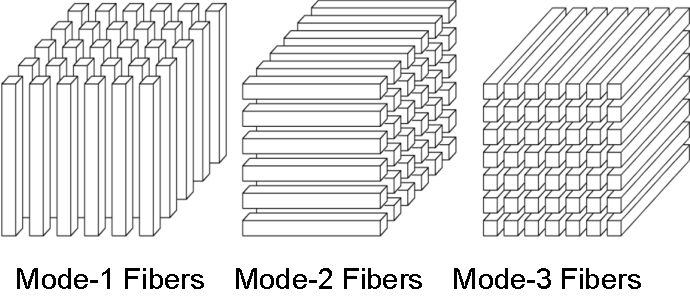
\includegraphics{fibers}}

\vfill

A tensor can be decomposed into the \emph{fibers} of each mode \\
(fibers are vectors -- fix all indices but one)

\end{center}

\end{frame}

\begin{frame}
\frametitle{Matricized Tensors}

\begin{center}

\scalebox{.25}{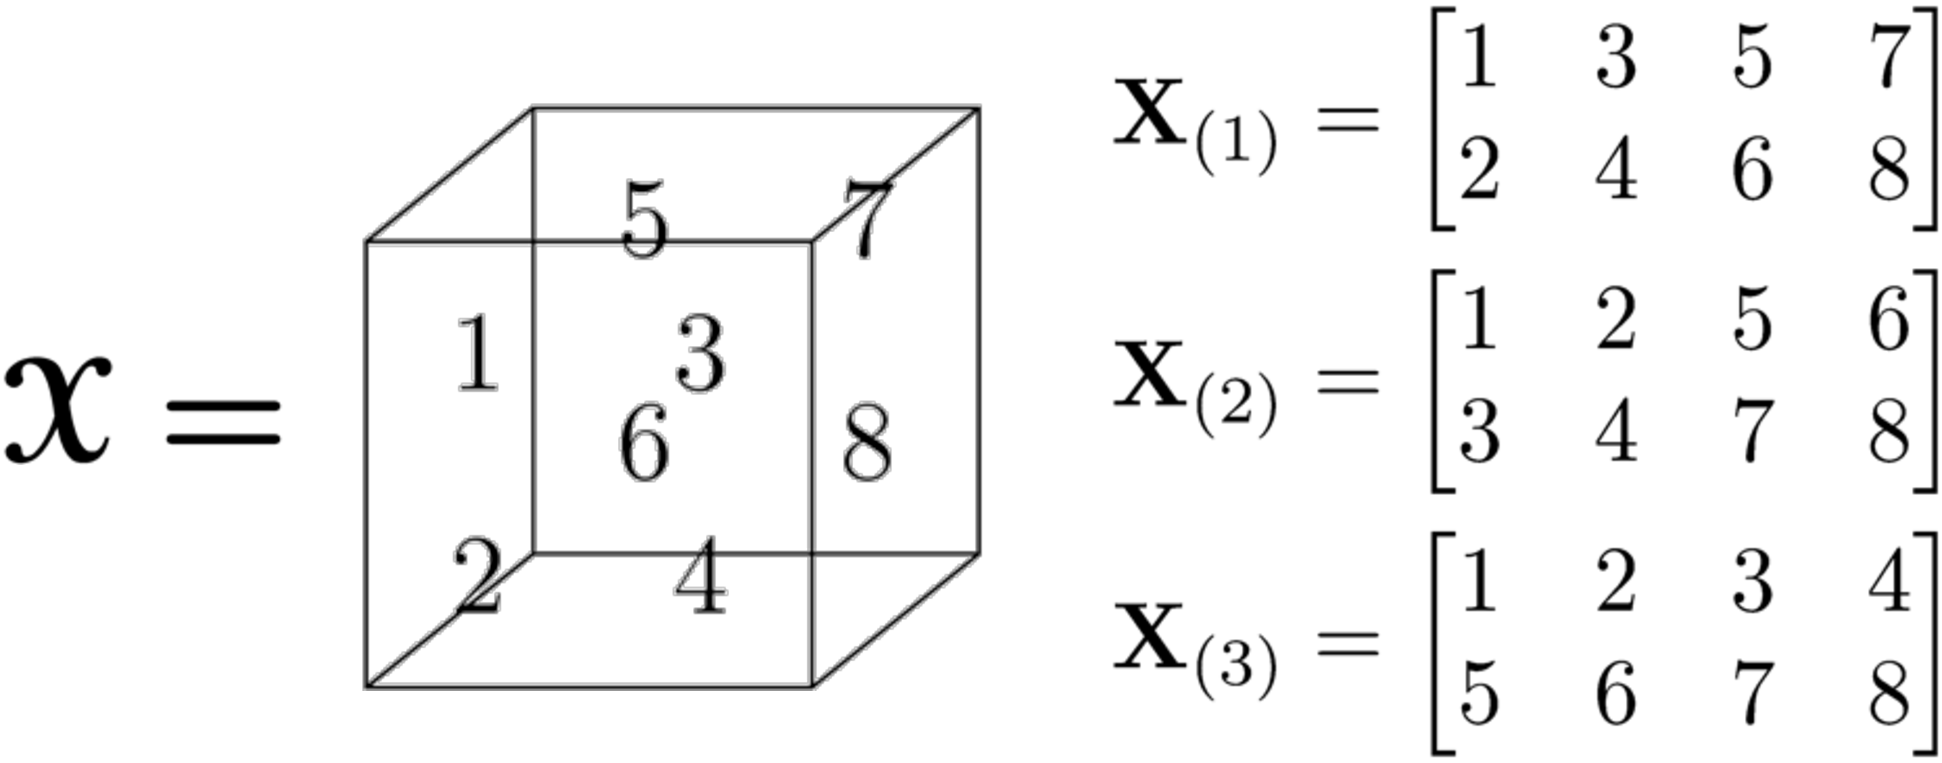
\includegraphics{unfoldings}}

\vfill

A tensor can be reshaped into a matrix, \\ 
called a \emph{matricized tensor} or \emph{unfolding}, for a given mode, \\
where each column is a fiber

\end{center}

\end{frame}

\begin{frame}
\frametitle{Sequential Communication Lower Bound}

\begin{theorem}
For sufficiently large $I$, any sequential MTTKRP algorithm performs at least
\begin{equation*}
\Omega\left(\frac{NIR}{M^{1-1/N}}\right)
\end{equation*}
loads and stores to/from slow memory.
\end{theorem}

\vfill

\small
\begin{itemize}
	\item $N$ is the number of modes
	\item $I$ is the number of tensor entries
	\item $R$ is the rank of the CP model
	\item $M$ is the size of the fast memory
\end{itemize}


\end{frame}

\begin{frame}
\frametitle{Communication-Optimal Sequential Algorithm (3D)}

\begin{columns}

\begin{column}{.55\textwidth}

\newcommand{\matdim}{4}
\newcommand{\mat}{\draw[black,shift={(-.5,-.5)}] (0,0) grid (\matdim,\matdim);}
\newcommand{\highlight}{gray!50}

\begin{center}
\begin{tikzpicture}[x={(-0.5cm,-0.4cm)}, y={(1cm,0cm)}, z={(0cm,1cm)},every node/.append style={transform shape},scale=.8]

% highlight tensor block and factor matrix subcolumns (do first to put in background)
% front face
\begin{scope}[canvas is yz plane at x=.5,shift={(1.5,-1.5)}]
	% highlight front face of tensor block
	\draw[dashed,fill=\highlight,shift={(0,0)}] (0,0) rectangle (-1,-1);
	\node[draw=none] at (-1.25,-.5) {\small $b$};
	\node[draw=none] at (-.5,-1.25) {\small $b$};
	% highlight block of 1st factor matrix
	\draw[fill=\highlight,shift={(-2.5,0)},xscale=.5] (0,0) rectangle (-1,-1);
	% highlight block of 2nd factor matrix
	\draw[fill=\highlight,shift={(0,-2.5)},yscale=.5] (0,0) rectangle (-1,-1);
	\only<2>{
	% highlight subcolumn of 1st factor matrix
	\draw[densely dotted,thick,shift={(-2.8,0)}] (0,0) -- (0,-1);
	% highlight subcolumn of 2nd factor matrix
	\draw[densely dotted,thick,shift={(0,-2.8)}] (0,0) -- (-1,0);
	}
\end{scope}
% right face
\begin{scope}[canvas is zx plane at y=(\matdim-.5),rotate=-90,shift={(.5,-4)}]
	% highlight block of 3rd factor matrix
	\draw[fill=\highlight,yscale=.5] (0,0) rectangle (-1,-1);
	\only<2>{
	% highlight subcolumn of 3rd factor matrix
	\draw[densely dotted,thick,shift={(0,-.3)}] (0,0) -- (-1,0);
	}
\end{scope}
% right face, but in middle of tensor
\begin{scope}[canvas is zx plane at y=1.5,rotate=-90,shift={(-.5,-2.5)}]
	% highlight right face of tensor block
	\draw[dashed,fill=\highlight] (0,0) rectangle (1,1);
	\node[draw=none] at (.75,-.2) {\small $b$};
\end{scope}
% top face, but in middle of tensor
\begin{scope}[canvas is yx plane at z=-1.5,yscale=-1,rotate=0,shift={(.5,-.5)}]
	\draw (0,0) node {\LARGE $\cdot$};
	% highlight top face of tensor block
	\draw[dashed,fill=\highlight] (0,0) rectangle (1,1);
\end{scope}

% draw tensor
% front face
\begin{scope}[canvas is yz plane at x=.5,rotate=-90]
	\mat
\end{scope}
% top face
\begin{scope}[canvas is yx plane at z=.5,yscale=-1,rotate=0]
	\mat
\end{scope}
% right face
\begin{scope}[canvas is zx plane at y=(\matdim-.5),rotate=180]
	\mat
\end{scope}

% draw factor matrices
% front face
\begin{scope}[canvas is yz plane at x=.5,shift={(1.5,-1.5)}]
	% draw 1st factor matrix
	\draw[shift={(-2.5,0)},xscale=.5] (0,-2) grid (-1,2);
	\node[draw=none] at (-3.5,0) {$\Mn{U}{1}$};
	% draw 2nd factor matrix
	\draw[shift={(0,-2.5)},yscale=.5] (-2,0) grid (2,-1);
	\node[draw=none] at (0,-3.5) {$\Mn{M}{2}$};
\end{scope}
% right face
\begin{scope}[canvas is zx plane at y=(\matdim-.5),rotate=-90,shift={(1.5,-1.5)}]
	% draw 3nd factor matrix
	\draw[shift={(0,-2.5)},yscale=.5] (-2,0) grid (2,-1);
	\node[draw=none] at (0,-3.5) {$\Mn{U}{3}$};
\end{scope}


\end{tikzpicture}
\end{center}

\end{column}
\begin{column}{.45\textwidth}

\footnotesize
\begin{enumerate}
	\item Loop over $b\times \cdots \times b$ blocks of the tensor
	\uncover<2>{\item With block in memory, loop over subcolumns of input factor matrices, updating corresponding subcolumn of output matrix}
\end{enumerate}

\vfill

\footnotesize
\begin{itemize}
	\uncover<2>{\item choose $b \approx M^{1/N}$}
\end{itemize}

\end{column}

\end{columns}

\end{frame}

\begin{frame}
\frametitle{Theoretical Comparisons}

\begin{center}
\renewcommand{\arraystretch}{2}
\begin{tabular}{|c|ccc|}
\hline
& \textbf{Lower Bound} & \textbf{New Algorithm} & \textbf{Standard (MM)} \\
\hline
\textbf{Flops} & - & $NIR$ & $2IR$ \\
\textbf{Words} & $\Omega\left( \frac{NIR}{M^{1-1/N}} \right)$ & $O\left( I+\frac{NIR}{M^{1-1/N}} \right)$ & $O\left( I+\frac{IR}{M^{1/2}} \right)$ \\
\textbf{Temp Mem} & - & - & $\frac{IR}{I_n}$ \\
\hline
\end{tabular}
\end{center}

\vfill
\pause

\begin{itemize}
	\item New algorithm performs $N/2$ more flops than standard
	\item For relatively small $R$, $I$ term dominates communication
	\begin{itemize}
		\item we expect this to be the typical case in practice
	\end{itemize}
	\item For relatively large $R$, new algorithm communicates less
	\begin{itemize}
		\item better exponent on $M$
	\end{itemize}
\end{itemize}

\end{frame}

\begin{frame}
\frametitle{MTTKRP Loop Nest}

\begin{algorithmic}
\For{$i_1=1$ to $I_1$}
	\ForDots
		\For{$i_N=1$ to $I_N$}
			\For{$r=1$ to $R$}
				\State \footnotesize $\Mn{M}{n}(i_n,r) \plusequals \T{X}(i_1,\dots,i_N) * \Mn{U}{1}(i_1,r) * \cdots * \Mn{U}{N}(i_N,r)$
			\EndFor
		\EndFor
	\EndForDots
\EndFor
\end{algorithmic}

\vfill

\begin{center}
$\Large \Delta= \quad\quad$
\begin{tabular}{c|cccccc}
& $i_1$ & $\cdots$ & $i_n$ & $\cdots$ & $i_N$ & $r$ \\
\hline 
$\Mn{U}{1}$ & 1 & & & & & 1 \\
$\vdots$ & & $\ddots$ & & & & $\vdots$ \\
$\Mn{M}{n}$ & & & 1 & & & 1 \\ 
$\vdots$ & & & & $\ddots$ & & $\vdots$ \\
$\Mn{U}{N}$ & & & & & 1 & 1 \\
$\T{X}$ & 1 & $\cdots$ & 1 & $\cdots$ & 1 & 
\end{tabular}
\end{center}

\end{frame}

\end{document}
